%-------------------------------------------------------------------------------
%	CAPITOLO 28
%-------------------------------------------------------------------------------

\chapter{Uno stronzo nella pentola}
Il signor \index[Personaggi]{Camerani Matteo (farmacista)}Matteo C.\:.\:.\footnote{\textbf{Matteo Camerani} fu un farmacista e fu figlio di  \index[Personaggi]{Camerani dott. Giannantonio (governatore)}Giannantonio Camerani, avvocato, governatore e Giudice di Pace, che a sua volta era figlio di \index[Personaggi]{Camerani Matteo (fattore)}Matteo Camerani, fattore della famiglia Spreti che aveva sposato la sorella di \index[Personaggi]{Monti Vincenzo}Vincenzo Monti, \index[Personaggi]{Monti Maria Cristina}Maria Cristina. Può sembrare confusionaria la genealogia ma è di fatto: Matteo (fattore), Giannantonio (governatore), Matteo (farmacista), Giovan Antonio} aveva fatto scodellare la minestra per sé, la moglie, ed i 4 figli e con la moglie cominciarono a soffiare sulle prime cucchiaiate perché si raffreddasse.\\
\indent I ragazzi erano a tavola meno uno, guardavano in giro e non mangiavano.\\
\indent Matteo, visto il posto vuoto: <<Dov'è \index[Personaggi]{Camerani Giovan Antonio}Giov Antonio...?>>\\
\indent I ragazzi zitti e poi: <<Un'iè\footnote{<<Non c'è>>}>>.\\
\indent Matteo\index[Personaggi]{Camerani Matteo (farmacista)}, al servitore: <<Galli val a ciamé, dov'è?\footnote{<<Vai a chiamarlo, dov'è?>>}>>\\
\indent Ragazzi: <<L'è a là fura!\footnote{<<È là fuori!>>}>>\\
\indent Matteo\index[Personaggi]{Camerani Matteo (farmacista)}: <<Perché non mangiate!>>\\
\indent I ragazzi zitti.\\
\indent Matteo\index[Personaggi]{Camerani Matteo (farmacista)}:  <<Magnì... av deg dal scòpul\footnote{<<Mangiate... vi dò delle scopole>> (scapaccioni)}>>.\\
\indent I ragazzi tentano la fuga, ma sono fermati.\\
\indent Matteo\index[Personaggi]{Camerani Matteo (farmacista)}: <<Parchè an magnì?\footnote{<<Perché non mangiate?>>}>>\\

\indent I ragazzi timidamente: <<Parchè Vàn Antoni\index[Personaggi]{Camerani Giovan Antonio}... la mès un strònz in t'la pignata\footnote{<<Perché Giov Antonio ha messo uno stronzo nella pentola>>}>>.\\
\indent Matteo: <<Ahc! Vigliac!\footnote{<<Bleah! Vigliacco!>>}>> e buttò tutto all'aria.\\

\centerline{\rule{1.5cm}{0.4pt}}

\index[Personaggi]{Boari Attilio (farmacista)}Boari era farmacista col signor Matteo\index[Personaggi]{Camerani Matteo (farmacista)}. La mattina del sopracitato fatto, non si sentiva bene.\\
\indent Per rinforzarlo sulle 11 gli portarono una tazza di buon brodo... di quello...\\
\indent Torse la bocca e poi: <<Cos'al ste brod. L'ha un fiè!\footnote{<<Cos'ha questo brodo? Fa una certa puzza!>>}>>\\
\indent Ma lo trangugiò egualmente... come ricostituente sostanzioso. I suoi clienti possano ritenersi vendicati... se da lui hanno avuto delle medicine amare!

 \begin{figure}[htb]
    \centering
    %\vspace{-0.7cm}
    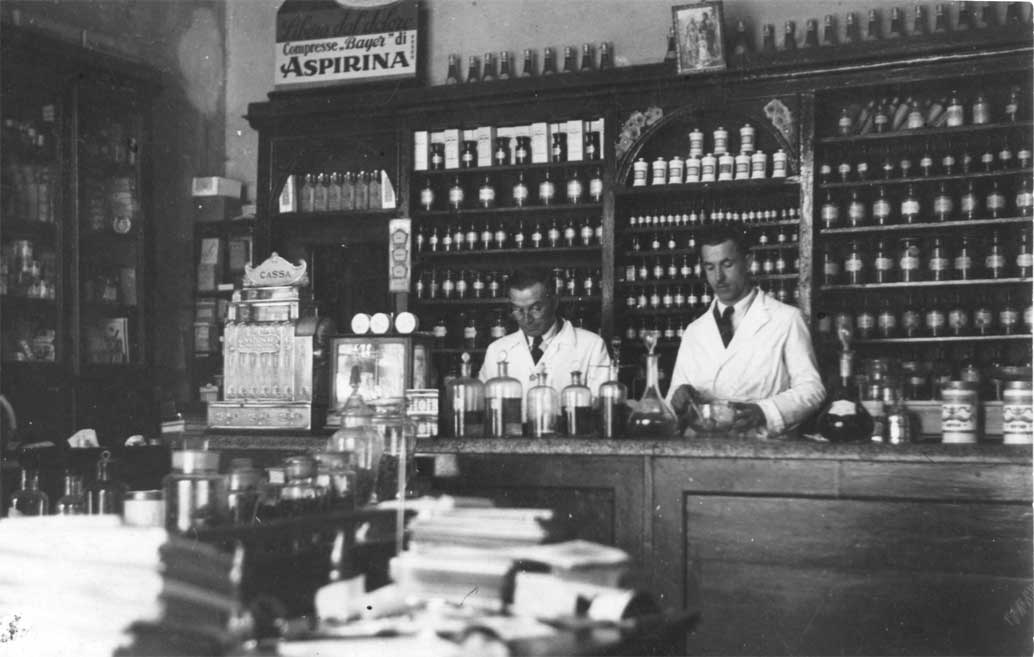
\includegraphics[width=\textwidth]{internofarmacia}
    \caption{L'interno della \index[Luoghi]{Farmacia Comunale}farmacia che era appartenuta ad \index[Personaggi]{Boari Attilio (farmacista)}\textbf{Attilio Boari}, diventata comunale dopo la sua morte. Nella foto vi sono i gestori succeduti a Boari, \textbf{Domenico Stella}\index[Personaggi]{Stella dott. Domenico} e \textbf{Nando Isani}\index[Personaggi]{Isani Nando}.\label{fig:internofarmacia}}
    %\vspace{-0.3cm}
\end{figure}


























